\section{Design Challenges: Performance, State, Consistency, and Security}
\label{sec:challenges}

Each generational leap in agent frameworks, from first-generation tool chains to fifth-generation autonomous agents, has exposed new systemic problems that neither the model itself nor ad hoc engineering workarounds can fully resolve.
This section examines five cross-cutting design challenges through a uniform lens: (1)~we describe a concrete scenario that illustrates the problem; (2)~we analyze the root cause; (3)~we survey current solutions; and (4)~we draw an explicit analogy to a well-studied problem in classical computer architecture.
Throughout, we trace each challenge back to the ICA layers (Section~\ref{sec:icam}) and the quantitative laws (Section~\ref{sec:laws}), arguing that the dual-plane architecture introduced in Section~\ref{sec:framework} is not merely an organizational convenience but a \emph{necessary} structural response to these challenges.


%% ---------- Latency, Throughput, Cost ----------
\subsection{The Latency--Throughput--Cost Trilemma}

\subsubsection{Scenario}
Consider a code agent assisting a developer in fixing a bug that spans ten files.
The agent must read multiple files (each read triggers a model inference call), understand the code structure, locate the fault, modify the code, run tests, inspect the results, and iterate.
The entire workflow may involve 20--50 model calls, and the per-call latency directly determines the developer's wait time.
If a single call costs 2~seconds, the end-to-end latency can easily exceed one minute.
If the serving provider provisions additional GPUs to reduce per-call latency, the cost per invocation rises proportionally.
Conversely, if the provider increases batch sizes to amortize cost and improve throughput, individual requests queue longer, increasing latency.
This is the \emph{latency--throughput--cost trilemma}: reducing latency demands more resources (higher cost), improving throughput demands larger batches (higher latency), and controlling cost demands fewer resources (higher latency and lower throughput).

\subsubsection{Root Cause}
The root cause lies in a structural asymmetry inherent to autoregressive LLM serving.
The \textbf{prefill} phase is \emph{compute-bound}: the entire input sequence must be processed in one forward pass, keeping GPU compute units fully occupied, with FLOPS as the bottleneck.
The \textbf{decode} phase is \emph{memory-bandwidth-bound}: generating each new token requires reading the full model weights and the current KV cache, effectively streaming all parameters from memory on every clock cycle~\cite{gholami2024memorywall}.
Gholami et al.\ quantify this imbalance: peak FLOPS grow at $3.0\times$ every two years, while DRAM bandwidth improves at only $1.6\times$ over the same period~\cite{gholami2024memorywall}.

Because the two phases demand fundamentally different hardware resources, co-scheduling them in the same batch inevitably leaves some resource underutilized: prefill monopolizes compute while decode stalls on memory bandwidth.
Agent workloads exacerbate this problem.
Multiple sub-agents issue concurrent requests whose context lengths vary wildly: one may read a single function while another must ingest an entire repository, rendering static batching strategies inefficient.

\subsubsection{Current Solutions}
The research community has responded at multiple levels.

\paragraph{Scheduling-level optimizations.}
ORCA~\cite{orca2022} introduces \emph{iteration-level scheduling}: rather than waiting for an entire sequence to complete before admitting new requests, the scheduler checks after every decode step whether a new request can join the running batch, significantly improving GPU utilization.
DistServe~\cite{zhong2024distserve} goes further by \emph{disaggregating} prefill and decode onto separate GPU groups, allowing each group to be independently optimized: high-FLOPS GPUs for prefill, high-bandwidth GPUs for decode.
Sarathi-Serve~\cite{agrawal2024sarathi} introduces stall-free scheduling via \emph{chunked prefill}, which slices long inputs into fixed-size chunks and interleaves them with decode tasks, eliminating stalls caused by waiting for large prefills to complete.

\paragraph{Memory management optimizations.}
vLLM~\cite{kwon2023pagedattention,vllm_docs_2026} employs PagedAttention to organize the KV cache into fixed-size pages mapped through a block table to non-contiguous physical memory, enabling on-demand allocation and sharing of KV cache.
SGLang~\cite{sglang2024,sglang_docs_2026} uses RadixAttention to organize request prefixes in a radix tree, automatically identifying and reusing shared-prefix KV cache entries.
TGI~\cite{tgi_docs_2026} and TensorRT-LLM~\cite{tensorrtllm_docs_2026} provide production-grade implementations of continuous batching and paged KV management.
vAttention~\cite{prabhu2024vattention} offers an alternative approach: leveraging OS-level contiguous virtual memory with dynamic growth to support standard attention kernels directly, bypassing the need for specialized PagedAttention kernels.

\subsubsection{Analogy to Classical Architecture}
This challenge is a direct analog of the classical \emph{memory wall}.
Since the 1980s, CPU speeds have improved at roughly 50\% per year while DRAM latency has improved at only 7\% per year~\cite{hennessy2017quantitative}.
The architectural response, including multi-level caches (L1/L2/L3), hardware prefetching, and write buffers, maps directly onto LLM serving: KV cache tiering corresponds to cache hierarchy, prefix caching to instruction cache sharing, and asynchronous decoding to write buffering.
The familiar response-time--throughput trade-off in time-sharing operating systems is also analogous: interactive tasks demand low response time (low latency) while batch tasks demand high throughput (large batches), and the scheduler must balance both~\cite{ostep_2023}.

Within ICA, this trilemma primarily spans L1 (physical execution) and L2 (inference serving).
Law~I (Section~\ref{sec:law1}) quantifies the cache-side of this trade-off: the KV cache hit rate $H$ directly determines the achievable speedup, and any scheduling or memory management optimization can be understood as an attempt to maximize $H$ under the trilemma's constraints.


%% ---------- State Management ----------
\subsection{State Management and Cross-Session Consistency}

\subsubsection{Scenario}
Suppose a user works with the same agent over three consecutive days to build a project.
On Day~1, the agent learns that the user prefers TypeScript over JavaScript.
On Day~2, the user asks the agent to refactor the codebase; the agent must respect the preference learned on Day~1 while correctly understanding the current state of the code.
On Day~3, the user discovers a new bug, and the agent must recall modifications made on both previous days (the bug may have been introduced by those very changes) while reasoning about the latest project state.
To complicate matters further, suppose the user runs two agent instances concurrently on Day~2: one performing the refactor and another writing tests.
Both agents may modify the same file, creating a conflict.

\subsubsection{Root Cause}
A traditional CPU is a \emph{stateless} executor: given the same inputs and register state, the output is deterministic and reproducible.
Intelligent systems, by contrast, must \emph{persist} state across sessions: user preferences (``I prefer TypeScript''), task history (``yesterday we refactored the authentication module''), and external-world changes (``three new files were added to the repository'').
Once persistent state is introduced, at least three categories of problems inevitably arise:

\begin{enumerate}[nosep]
\item \textbf{Concurrent access to shared memory.}
When multiple agents read and write shared memory simultaneously, how do we guarantee consistency?
This is analogous to race conditions in multi-threaded programming.

\item \textbf{Delayed commits and conflict resolution.}
Agent~A modifies a file but has not yet committed the change; Agent~B begins modifying the same file based on the old version.
Detecting and resolving such conflicts mirrors optimistic concurrency control in distributed systems.

\item \textbf{Memory staleness.}
The fact ``the project uses React'' learned three days ago may be obsolete because the project has since migrated to Vue.
Determining whether a memory is still valid is analogous to cache invalidation.
\end{enumerate}

\subsubsection{Current Solutions}
The LongMemEval benchmark~\cite{longmemeval2024} demonstrates that long-term memory is not simply ``storing more chat logs'' but requires four distinct capabilities: information extraction (distilling key facts from conversation), temporal reasoning (understanding event ordering), knowledge updating (revising old memories when new information conflicts), and refusal (declining to answer when memory is insufficient).

MemGPT~\cite{memgpt2023} borrows the paging and swap-in/swap-out mechanisms of OS virtual memory to manage context, dividing it into ``main memory'' (the active context window) and ``external storage'' (long-term memory in a vector database), with explicit edit and retrieve operations to move information between the two.
MemoryOS~\cite{memoryos2025} abstracts memory management as an OS memory management module, implementing structured memory encoding, retrieval, and update.
A-MEM~\cite{amem2025} proposes agentic memory management: memories are not passively stored strings but ``active entities'' whose creation, update, and deletion are governed by the agent itself.
Letta~\cite{letta_stateful_2026} (formerly the MemGPT project) further elevates ``stateful agents'' to a core abstraction, explicitly separating conversational state, core memory, and archival memory.

From a distributed systems perspective, at least three state types must be distinguished~\cite{raft2014,spanner2012,cap2002}:
\begin{enumerate}[nosep]
\item \textbf{Ephemeral state:} intermediate results of the current inference step, analogous to CPU registers; no persistence required.
\item \textbf{Session state with causal ordering:} message passing and state transfer among agents within the same task, requiring causal consistency guarantees analogous to those in distributed systems~\cite{raft2014}.
\item \textbf{Committed state with full auditability and replay:} permanent modifications to files, databases, or external systems, analogous to a database transaction's commit point, supporting audit and rollback~\cite{spanner2012}.
\end{enumerate}

\subsubsection{Temporal Decay in Long-Running Agents}
Critically, the time horizon of agent execution is expanding from minutes to hours and even days.
Recent industrial practice shows that agents can autonomously run for over seven hours to complete complex tasks~\cite{anthropic2026agenticreport}.
Such cross-hour and cross-day execution introduces additional temporal decay challenges: the attention decay function $\beta(L)$ is no longer solely a function of context position but also depends on session duration and cross-step state accumulation.
This means the three-way state classification above acquires a time dimension: cross-hour execution requires session-persistent KV caches (L2), context window management must support working-set restoration across checkpoints (L3), and the governance layer must define periodic checkpointing and human-recovery protocols (L5).
Law~II (Section~\ref{sec:law2}), as currently formulated, does not capture this temporal dimension, an important direction for future work.

\subsubsection{Analogy to Classical Architecture}
These challenges map directly onto \emph{virtual memory and distributed consistency} in classical systems.
OS virtual memory uses page tables to map virtual to physical addresses and provides swap mechanisms to create the illusion of unbounded memory, analogous to context management in agent systems.
Distributed file systems such as GFS and Spanner~\cite{spanner2012} use Paxos/Raft~\cite{raft2014} consensus protocols to guarantee multi-replica consistency, analogous to consistency in multi-agent shared memory.
The CAP theorem~\cite{cap2002} states that consistency, availability, and partition tolerance cannot be simultaneously achieved; agent memory management faces the same trade-off: strong consistency (synchronizing all replicas before acknowledging each operation) versus eventual consistency (tolerating brief inconsistency in exchange for lower latency).

Within ICA, this challenge primarily spans L3 (context management) and L5 (orchestration).
The dual-plane architecture naturally separates the problem: the probabilistic execution plane manages the working context (what to remember and what to forget), while the deterministic control plane enforces consistency guarantees and conflict-resolution protocols.


%% ---------- Interface Drift ----------
\subsection{Interface Drift and Version Compatibility}

\subsubsection{Scenario}
An agent is configured to manage a code repository via the GitHub API.
One day, GitHub updates the API from v3 to v4: the endpoint \texttt{repos/:owner/:repo/pulls} returns a new response format, adds pagination parameters, and removes several fields.
The agent's tool calls begin returning errors or failing to parse responses.
A more subtle scenario: the agent's prompt template relies on the model producing output in a specific format (e.g., ``always respond in JSON''), but a model upgrade subtly changes the output style, causing the downstream parser to crash repeatedly.
Similar problems arise when MCP servers update their capability descriptions, when skill packs change their interfaces, or when memory file formats undergo version upgrades.

\subsubsection{Root Cause}
Classical computer systems achieve scalability in large part because their core interfaces, including ISA, ABI, system calls, and file formats, remain \emph{stable over decades}.
The x86 instruction set has maintained backward compatibility from the 8086 (1978) through the latest processors in 2026; the POSIX standard, established in 1988, has preserved the semantics of \texttt{read()}/\texttt{write()}/\texttt{fork()} with almost no change~\cite{ostep_2023}.
This stability allows upper-layer software to be built with confidence that the ground beneath it will not shift unexpectedly.

The current agent ecosystem, by contrast, suffers from severe \emph{interface drift}.
At least four sources of drift can be identified:
\begin{enumerate}[nosep]
\item \textbf{Model version drift:} a model upgrade may change the output format for the same prompt.
\item \textbf{Tool schema drift:} external APIs may update their interface descriptions and response formats without warning~\cite{mcp_intro_2026}.
\item \textbf{Protocol drift:} protocols such as MCP and A2A are themselves under rapid iteration~\cite{agentprotocols2025,google_a2a_2025}.
\item \textbf{Skill pack drift:} reusable agent skills may behave differently across projects or model versions.
\end{enumerate}

\subsubsection{Current Solutions}
OpenAI Codex provides project-level stability anchors through AGENTS.md~\cite{openai_codex_agents_md_2026} and the Skills mechanism~\cite{openai_codex_skills_2026}: each skill pack carries explicit version numbers and compatibility declarations.
Claude Code achieves similar functionality through CLAUDE.md~\cite{anthropic_claudecode_memory_2026}.
Interoperability protocols, including MCP~\cite{mcp_intro_2026} for model--tool communication and A2A~\cite{google_a2a_2025} for agent--agent interaction, are attempting to establish standardized interfaces.
The A2A protocol, built on JSON-RPC 2.0 over HTTP, defines standard workflows for agent discovery, capability negotiation, and task delegation~\cite{google_a2a_2025}.
However, these protocols are themselves evolving rapidly and have not yet achieved the stability of an ISA or POSIX.

\subsubsection{Analogy to Classical Architecture}
This challenge corresponds to \emph{ABI stability and version management} in classical systems.
Intel has maintained x86 backward compatibility for over 45~years; the Linux kernel has preserved system-call backward compatibility for over 30~years; even shared-library versioning has mature solutions (semantic versioning, symbol versioning).
Model-native computing architectures must develop their own ``version control discipline'': tool schemas need version numbers, model output formats need compatibility guarantees, skill packs need dependency management (analogous to npm's \texttt{package.json}), and memory files need format migration tools (analogous to database schema migration).

Within ICA, interface drift primarily affects L4 (semantic interface layer) and the L4--L5 boundary.
The deterministic control plane must maintain version-aware interface contracts that insulate the probabilistic execution plane from upstream changes, precisely the role that ABI stability plays in shielding application software from hardware evolution.


%% ---------- Security, Privacy, Least Privilege ----------
\subsection{Security, Privacy, and Least Privilege}

\subsubsection{Scenario}
A code agent is helping a developer process user data.
The agent must read database schemas that contain personally identifiable information (to understand the data model), modify code that handles user data, and run tests whose fixtures may include real user records.
During this process, the agent may: (1)~write sensitive data to log files or transmit it to a remote API (data exfiltration); (2)~be manipulated by a malicious code comment or file content into performing unintended actions via prompt injection (goal hijacking); (3)~use real user data in tests instead of synthetic fixtures (privacy violation).
Worse still: since the agent can execute arbitrary shell commands, a carefully crafted prompt injection could cause it to run \texttt{rm -rf /} or upload sensitive files to an external server.

\subsubsection{Root Cause}
Once an agent can read and write files, execute commands, browse the web, and query databases, it is no longer merely a language model but an \emph{agent} in the security sense: a principal with external action capability.
This introduces attack surfaces that classical software security does not cover:

\begin{enumerate}[nosep]
\item \textbf{Prompt injection.}
An attacker embeds malicious instructions in tool-returned data, file contents, or web pages to hijack the agent's behavior.
Unlike classical code injection (e.g., SQL injection), prompt injection exploits not a logic flaw but the model's inability to distinguish ``instructions from the user'' from ``instructions embedded in data''~\cite{debenedetti2025camel,owasp_agentic2026}.

\item \textbf{Privilege over-provisioning.}
Most current agents, when granted tool access, receive the tool's \emph{full} permission set (e.g., read/write access to the entire filesystem) rather than the minimum necessary privilege (e.g., read/write access only to specific project files).

\item \textbf{Memory taint propagation.}
A successful prompt injection can write malicious information into the agent's long-term memory; this ``tainted'' memory then influences the agent's behavior across all subsequent sessions, creating a persistent backdoor~\cite{aura2025}.
\end{enumerate}

\subsubsection{Current Solutions}
Industry and academia are constructing defenses along multiple dimensions.

\paragraph{Sandboxing.}
OpenAI Codex runs tasks by default inside an OS-enforced sandbox, where each task executes in an isolated container without access to the host filesystem or network~\cite{openai_codex_sandbox_2026}.
Claude Code operates in read-only mode by default, requiring explicit user authorization for any write operation~\cite{anthropic_claudecode_security_2026}.
Aura establishes independent sandboxes for each app agent on mobile devices and restricts the agent kernel's access to system resources~\cite{aura2025}.

\paragraph{Capability-based security models.}
CaMeL~\cite{debenedetti2025camel} applies the OS capability-security principle to defend against prompt injection: the agent cannot directly execute side-effecting operations but must obtain a ``temporary pass'' from a deterministic capability manager.
Each pass authorizes exactly one specific operation (e.g., ``read-only access to \texttt{src/main.py}'') and is consumed upon use.
This fundamentally eliminates the possibility of privilege escalation via prompt injection, because permissions are governed by deterministic code rather than a probabilistic model.

\paragraph{Approval and audit.}
Codex's approval policies~\cite{openai_codex_approvals_2026} allow developers to specify which operations require human confirmation (e.g., ``any \texttt{DELETE} operation must be approved'').
The Agents SDK's tracing mechanism~\cite{openai_codex_agentsdk_2026} records the full context of every tool call, supporting post-hoc audit and replay.

\paragraph{Formal security.}
IronClaw~\cite{ironclaw2025} proposes a formal framework for agent security that explicitly models the agent's behavior space and permission space, detecting out-of-bounds actions through static analysis and runtime monitoring.
Christodorescu et al.~\cite{agenticsecurity2025} argue that agent security must draw on the full experience of operating system security: least privilege, isolation, auditing, and fail-safe defaults.

\subsubsection{Analogy to Classical Architecture}
These challenges correspond to \emph{process security and permission management} in classical systems.
Unix security rests on three core concepts: (1)~user/kernel mode separation, where user programs cannot access hardware directly and must go through system calls~\cite{ostep_2023}; (2)~file permissions (rwx), where each file has explicit read, write, and execute permissions; (3)~root/non-root separation, where privileged operations require explicit elevation.
Agent security requires an analogous three-layer model: (1)~probabilistic-plane/deterministic-plane separation, where agents cannot directly execute side-effecting operations but must pass through the deterministic control plane's approval channel; (2)~tool capability annotations, where each tool carries explicit capability declarations and permission requirements; (3)~governance-layer privilege elevation, where high-risk operations require explicit authorization or human confirmation.

\subsubsection{Dual-Use Security Concerns}
It is important to recognize that agent capabilities are inherently dual-use.
The same capabilities that enable automated security auditing (defensive use) can also enable automated vulnerability discovery and exploitation (offensive use)~\cite{anthropic2026agenticreport}.
This means the deterministic control plane of a dual-plane architecture must not only constrain its own agents' behavior but also anticipate that adversaries possess equivalent dual-plane systems.
Anthropic's 2026 agentic security report predicts that ``agentic cyber defense systems'' will operate at machine speed~\cite{anthropic2026agenticreport}, implying that the L5 governance layer's primitives must incorporate adversarial scenarios into their threat models from the outset.

Within ICA, security spans all six layers but concentrates at L4 (tool capability annotations and call audits) and L5 (permission approval and failure recovery).
The dual-plane architecture is essential here: the probabilistic plane handles the reasoning needed to interpret user intent, while the deterministic plane enforces the non-negotiable security invariants.


%% ---------- Governance ----------
\subsection{Governance as a First-Class Architectural Concern}

\subsubsection{The Core Problem}
ArbiterOS~\cite{arbiteros2025} identifies the fundamental crisis in agent engineering as a structural contradiction: developers instinctively apply \emph{deterministic software thinking} to drive a \emph{probabilistic processor}.
In traditional software engineering, code behavior is deterministic: identical inputs produce identical outputs, tests can cover all branches, and bugs can be caught with assertions.
Agent behavior, however, is driven by a probabilistic model: the same prompt may yield different outputs across invocations, tests cannot cover all possible reasoning paths, and ``bugs'' manifest as hallucinations or instruction-following failures that resist detection by traditional assertions.

Aura~\cite{aura2025} further demonstrates that once agents enter the OS and mobile environments, permission management (does the agent have access to the contacts list?), authentication (is the caller the genuine user or an attacker?), semantic input pollution (can a malicious SMS hijack the agent?), and memory taint propagation (how is tainted memory cleaned?) all become \emph{kernel-level} concerns, no longer merely application-layer vulnerabilities but foundational security issues for the entire system architecture.

Figure~\ref{fig:challenge_heatmap} maps each challenge to the ICA layers it impacts most, showing primary, secondary, and tertiary impact levels across the full stack.
\begin{figure}[h]
\centering
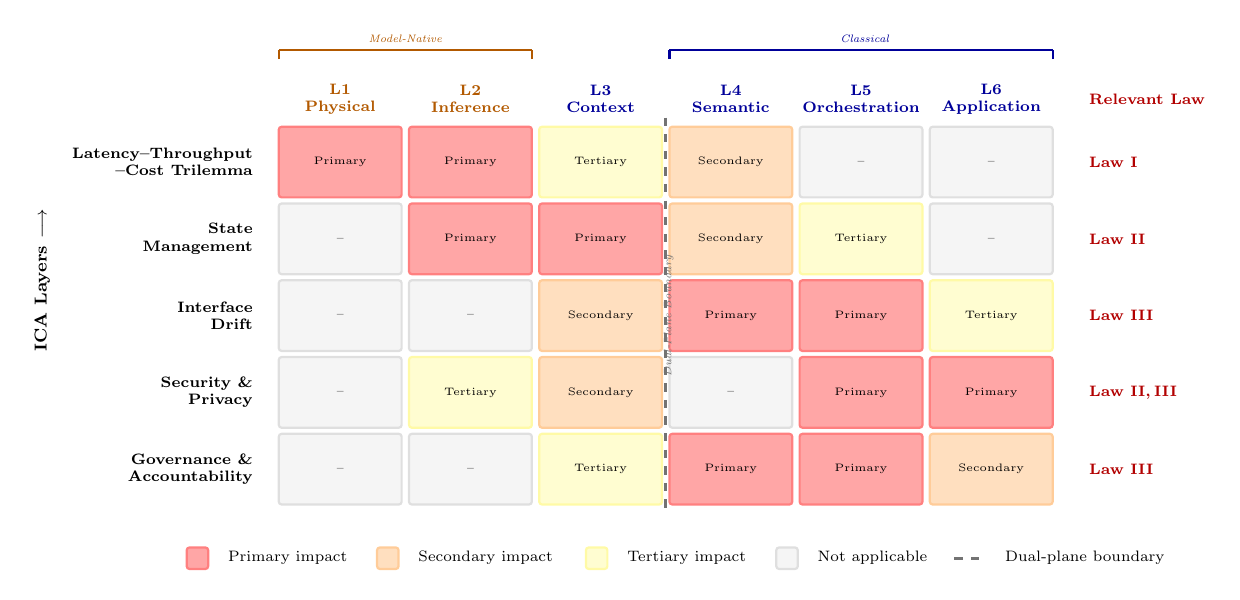
\begin{tikzpicture}[
    scale=0.78,
    transform shape,
    % --- cell styles by severity ---
    primary/.style={fill=red!35, draw=red!50, thick, rounded corners=1pt},
    secondary/.style={fill=orange!25, draw=orange!40, thick, rounded corners=1pt},
    tertiary/.style={fill=yellow!18, draw=yellow!35, thick, rounded corners=1pt},
    notapplic/.style={fill=gray!8, draw=gray!25, thick, rounded corners=1pt},
    % --- header styles ---
    colhead/.style={font=\scriptsize\bfseries, align=center, text width=1.8cm},
    rowhead/.style={font=\scriptsize\bfseries, align=right, anchor=east, text width=3.4cm},
    lawlabel/.style={font=\scriptsize\bfseries, align=center, anchor=west},
    celltxt/.style={font=\tiny, align=center},
    % --- axis labels ---
    axlbl/.style={font=\footnotesize\bfseries},
]

% === dimensions ===
\def\cellw{2.0}   % column width (cm)
\def\cellh{1.15}   % row height (cm)
\def\colsep{0.12}  % horizontal gap between cells
\def\rowsep{0.10}  % vertical gap between cells
\def\rowoff{5}     % number of rows minus 1 (0-indexed)
\def\coloff{5}     % number of cols minus 1 (0-indexed)

% === origin offsets ===
\def\xstart{4.0}   % left edge of first data column
\def\ystart{6.2}    % top edge of first data row

% === column headers (L1--L6) ===
% Use explicit two-line labels to prevent word-break hyphenation
\pgfmathsetmacro{\cx}{\xstart + 0*(\cellw+\colsep) + \cellw/2}
\node[colhead, text=orange!70!black] at (\cx, \ystart + 0.45) {L1\\Physical};
\pgfmathsetmacro{\cx}{\xstart + 1*(\cellw+\colsep) + \cellw/2}
\node[colhead, text=orange!70!black] at (\cx, \ystart + 0.45) {L2\\Inference};
\pgfmathsetmacro{\cx}{\xstart + 2*(\cellw+\colsep) + \cellw/2}
\node[colhead, text=blue!60!black] at (\cx, \ystart + 0.45) {L3\\Context};
\pgfmathsetmacro{\cx}{\xstart + 3*(\cellw+\colsep) + \cellw/2}
\node[colhead, text=blue!60!black] at (\cx, \ystart + 0.45) {L4\\Semantic};
\pgfmathsetmacro{\cx}{\xstart + 4*(\cellw+\colsep) + \cellw/2}
\node[font=\scriptsize\bfseries, align=center, text width=2.2cm, text=blue!60!black] at (\cx, \ystart + 0.45) {L5\\Orchestration};
\pgfmathsetmacro{\cx}{\xstart + 5*(\cellw+\colsep) + \cellw/2}
\node[colhead, text=blue!60!black] at (\cx, \ystart + 0.45) {L6\\Application};

% === column sub-headers: plane labels (raised slightly) ===
\pgfmathsetmacro{\modelnativex}{\xstart + \cellw + \colsep/2}
\node[font=\tiny\itshape, orange!70!black, anchor=south] at (\modelnativex, \ystart + 1.25) {Model-Native};
\pgfmathsetmacro{\classicalx}{\xstart + 3*(\cellw+\colsep) + 1.5*\cellw + 1.5*\colsep}
\node[font=\tiny\itshape, blue!60!black, anchor=south] at (\classicalx, \ystart + 1.25) {Classical};

% === row headers (5 challenges) ===
\pgfmathsetmacro{\rx}{\xstart - 0.3}
\pgfmathsetmacro{\ryA}{\ystart - 0*(\cellh+\rowsep) - \cellh/2}
\pgfmathsetmacro{\ryB}{\ystart - 1*(\cellh+\rowsep) - \cellh/2}
\pgfmathsetmacro{\ryC}{\ystart - 2*(\cellh+\rowsep) - \cellh/2}
\pgfmathsetmacro{\ryD}{\ystart - 3*(\cellh+\rowsep) - \cellh/2}
\pgfmathsetmacro{\ryE}{\ystart - 4*(\cellh+\rowsep) - \cellh/2}
\node[rowhead] at (\rx, \ryA)
    {Latency--Throughput\\--Cost Trilemma};
\node[rowhead] at (\rx, \ryB)
    {State\\Management};
\node[rowhead] at (\rx, \ryC)
    {Interface\\Drift};
\node[rowhead] at (\rx, \ryD)
    {Security \&\\Privacy};
\node[rowhead] at (\rx, \ryE)
    {Governance \&\\Accountability};

% === heatmap cells ===
% Row 0: Latency/Cost -- Primary L1,L2; Secondary L4; Tertiary L3; NA L5,L6
\foreach \c/\sty in {0/primary, 1/primary, 2/tertiary, 3/secondary, 4/notapplic, 5/notapplic}{
    \pgfmathsetmacro{\xll}{\xstart + \c*(\cellw+\colsep)}
    \pgfmathsetmacro{\yll}{\ystart - \cellh}
    \draw[\sty] (\xll, \yll) rectangle +(\cellw, \cellh);
}
% Severity text inside cells
\foreach \c/\lab in {0/Primary, 1/Primary, 2/Tertiary, 3/Secondary, 4/--, 5/--}{
    \pgfmathsetmacro{\cx}{\xstart + \c*(\cellw+\colsep) + \cellw/2}
    \pgfmathsetmacro{\cy}{\ystart - \cellh + \cellh/2}
    \node[celltxt] at (\cx, \cy) {\lab};
}

% Row 1: State Mgmt -- Primary L2,L3; Secondary L4; Tertiary L5; NA L1,L6
\foreach \c/\sty in {0/notapplic, 1/primary, 2/primary, 3/secondary, 4/tertiary, 5/notapplic}{
    \pgfmathsetmacro{\xll}{\xstart + \c*(\cellw+\colsep)}
    \pgfmathsetmacro{\yll}{\ystart - 1*(\cellh+\rowsep) - \cellh}
    \draw[\sty] (\xll, \yll) rectangle +(\cellw, \cellh);
}
\foreach \c/\lab in {0/--, 1/Primary, 2/Primary, 3/Secondary, 4/Tertiary, 5/--}{
    \pgfmathsetmacro{\cx}{\xstart + \c*(\cellw+\colsep) + \cellw/2}
    \pgfmathsetmacro{\cy}{\ystart - 1*(\cellh+\rowsep) - \cellh + \cellh/2}
    \node[celltxt] at (\cx, \cy) {\lab};
}

% Row 2: Interface Drift -- Primary L4,L5; Secondary L3; Tertiary L6; NA L1,L2
\foreach \c/\sty in {0/notapplic, 1/notapplic, 2/secondary, 3/primary, 4/primary, 5/tertiary}{
    \pgfmathsetmacro{\xll}{\xstart + \c*(\cellw+\colsep)}
    \pgfmathsetmacro{\yll}{\ystart - 2*(\cellh+\rowsep) - \cellh}
    \draw[\sty] (\xll, \yll) rectangle +(\cellw, \cellh);
}
\foreach \c/\lab in {0/--, 1/--, 2/Secondary, 3/Primary, 4/Primary, 5/Tertiary}{
    \pgfmathsetmacro{\cx}{\xstart + \c*(\cellw+\colsep) + \cellw/2}
    \pgfmathsetmacro{\cy}{\ystart - 2*(\cellh+\rowsep) - \cellh + \cellh/2}
    \node[celltxt] at (\cx, \cy) {\lab};
}

% Row 3: Security & Privacy -- Primary L5,L6; Secondary L3; Tertiary L2; NA L1,L4
\foreach \c/\sty in {0/notapplic, 1/tertiary, 2/secondary, 3/notapplic, 4/primary, 5/primary}{
    \pgfmathsetmacro{\xll}{\xstart + \c*(\cellw+\colsep)}
    \pgfmathsetmacro{\yll}{\ystart - 3*(\cellh+\rowsep) - \cellh}
    \draw[\sty] (\xll, \yll) rectangle +(\cellw, \cellh);
}
\foreach \c/\lab in {0/--, 1/Tertiary, 2/Secondary, 3/--, 4/Primary, 5/Primary}{
    \pgfmathsetmacro{\cx}{\xstart + \c*(\cellw+\colsep) + \cellw/2}
    \pgfmathsetmacro{\cy}{\ystart - 3*(\cellh+\rowsep) - \cellh + \cellh/2}
    \node[celltxt] at (\cx, \cy) {\lab};
}

% Row 4: Governance -- Primary L4,L5; Secondary L6; Tertiary L3; NA L1,L2
\foreach \c/\sty in {0/notapplic, 1/notapplic, 2/tertiary, 3/primary, 4/primary, 5/secondary}{
    \pgfmathsetmacro{\xll}{\xstart + \c*(\cellw+\colsep)}
    \pgfmathsetmacro{\yll}{\ystart - 4*(\cellh+\rowsep) - \cellh}
    \draw[\sty] (\xll, \yll) rectangle +(\cellw, \cellh);
}
\foreach \c/\lab in {0/--, 1/--, 2/Tertiary, 3/Primary, 4/Primary, 5/Secondary}{
    \pgfmathsetmacro{\cx}{\xstart + \c*(\cellw+\colsep) + \cellw/2}
    \pgfmathsetmacro{\cy}{\ystart - 4*(\cellh+\rowsep) - \cellh + \cellh/2}
    \node[celltxt] at (\cx, \cy) {\lab};
}

% === Dual-plane boundary: thick dashed line between L3 and L4 ===
\pgfmathsetmacro{\bndx}{\xstart + 3*(\cellw+\colsep) - \colsep/2}
\pgfmathsetmacro{\bndtop}{\ystart + 0.15}
\pgfmathsetmacro{\bndbot}{\ystart - 4*(\cellh+\rowsep) - \cellh - 0.15}
\draw[very thick, dashed, black!55] (\bndx, \bndtop) -- (\bndx, \bndbot);

% Small label for the boundary
\pgfmathsetmacro{\bndmid}{(\bndtop + \bndbot)/2}
\node[font=\tiny\itshape, black!55, rotate=90, anchor=south] at (\bndx + 0.25, \bndmid)
    {Dual-Plane Boundary};

% === Right-margin annotation: quantitative law relevance ===
\pgfmathsetmacro{\lawx}{\xstart + 6*(\cellw+\colsep) + 0.35}

% Row 0: Latency/Cost -> Law I (Energy/Performance scaling)
\pgfmathsetmacro{\ry}{\ystart - 0*(\cellh+\rowsep) - \cellh/2}
\node[lawlabel, red!70!black] at (\lawx, \ry) {Law~I};

% Row 1: State Mgmt -> Law II (Memory/State consistency)
\pgfmathsetmacro{\ry}{\ystart - 1*(\cellh+\rowsep) - \cellh/2}
\node[lawlabel, red!70!black] at (\lawx, \ry) {Law~II};

% Row 2: Interface Drift -> Law III (Interface stability)
\pgfmathsetmacro{\ry}{\ystart - 2*(\cellh+\rowsep) - \cellh/2}
\node[lawlabel, red!70!black] at (\lawx, \ry) {Law~III};

% Row 3: Security & Privacy -> Law III + II
\pgfmathsetmacro{\ry}{\ystart - 3*(\cellh+\rowsep) - \cellh/2}
\node[lawlabel, red!70!black] at (\lawx, \ry) {Law~II,\,III};

% Row 4: Governance -> Law III
\pgfmathsetmacro{\ry}{\ystart - 4*(\cellh+\rowsep) - \cellh/2}
\node[lawlabel, red!70!black] at (\lawx, \ry) {Law~III};

% Right-margin column header
\node[font=\scriptsize\bfseries, red!70!black, anchor=west] at (\lawx, \ystart + 0.45)
    {Relevant Law};

% === Axis labels ===
\pgfmathsetmacro{\axleft}{\xstart - 3.6}
\pgfmathsetmacro{\axmid}{\ystart - 2*(\cellh+\rowsep)}
\node[axlbl, rotate=90, anchor=south] at (\axleft, \axmid)
    {ICA Layers $\longrightarrow$};

\pgfmathsetmacro{\axbotx}{\xstart + 2.5*(\cellw+\colsep)}
\pgfmathsetmacro{\axboty}{\ystart - 4*(\cellh+\rowsep) - \cellh - 0.5}
\node[axlbl, anchor=north] at (\axbotx, \axboty) {};

% === Legend (centred, items spaced so text doesn't overlap next box) ===
\def\legy{-1.0}
\def\legx{2.5}
% Each item: box(0.35) + gap(0.2) + text + gap(0.5) before next box
% "Primary impact" ~1.8cm, "Secondary impact" ~2.1cm, "Tertiary impact" ~1.7cm
% item spacing: 3.1cm apart

% Primary
\draw[primary] (\legx, \legy) rectangle +(0.35, 0.35);
\node[font=\scriptsize, anchor=west] at (\legx + 0.55, \legy + 0.175)
    {Primary impact\hspace{0.4em}};

% Secondary  (start at legx + 3.1)
\pgfmathsetmacro{\lx}{\legx + 3.1}
\draw[secondary] (\lx, \legy) rectangle +(0.35, 0.35);
\node[font=\scriptsize, anchor=west] at (\lx + 0.55, \legy + 0.175)
    {Secondary impact\hspace{0.4em}};

% Tertiary  (start at legx + 6.5)
\pgfmathsetmacro{\lx}{\legx + 6.5}
\draw[tertiary] (\lx, \legy) rectangle +(0.35, 0.35);
\node[font=\scriptsize, anchor=west] at (\lx + 0.55, \legy + 0.175)
    {Tertiary impact\hspace{0.4em}};

% Not applicable  (start at legx + 9.6)
\pgfmathsetmacro{\lx}{\legx + 9.6}
\draw[notapplic] (\lx, \legy) rectangle +(0.35, 0.35);
\node[font=\scriptsize, anchor=west] at (\lx + 0.55, \legy + 0.175)
    {Not applicable\hspace{0.4em}};

% Boundary legend entry  (start at legx + 12.5)
\pgfmathsetmacro{\lx}{\legx + 12.5}
\draw[very thick, dashed, black!55] (\lx, \legy + 0.175) -- ++(0.5, 0);
\node[font=\scriptsize, anchor=west] at (\lx + 0.7, \legy + 0.175)
    {Dual-plane boundary};

% Plane annotations along top
\pgfmathsetmacro{\modelleft}{\xstart}
\pgfmathsetmacro{\modelright}{\xstart + 2*\cellw + \colsep}
\pgfmathsetmacro{\classleft}{\xstart + 3*(\cellw+\colsep)}
\pgfmathsetmacro{\classright}{\xstart + 5*(\cellw+\colsep) + \cellw}
\pgfmathsetmacro{\bracetop}{\ystart + 1.1}

% Underbrace for model-native plane
\draw[thick, orange!70!black]
    (\modelleft, \bracetop) -- (\modelleft, \bracetop + 0.15);
\draw[thick, orange!70!black]
    (\modelright, \bracetop) -- (\modelright, \bracetop + 0.15);
\draw[thick, orange!70!black]
    (\modelleft, \bracetop + 0.15) -- (\modelright, \bracetop + 0.15);

% Underbrace for classical plane
\draw[thick, blue!60!black]
    (\classleft, \bracetop) -- (\classleft, \bracetop + 0.15);
\draw[thick, blue!60!black]
    (\classright, \bracetop) -- (\classright, \bracetop + 0.15);
\draw[thick, blue!60!black]
    (\classleft, \bracetop + 0.15) -- (\classright, \bracetop + 0.15);

\end{tikzpicture}
\caption{Challenge-to-ICA-layer impact heatmap. Each cell indicates the severity of a given challenge at the corresponding ICA layer: \textcolor{red!50}{\textbf{primary}} (direct, critical impact), \textcolor{orange!40}{\textbf{secondary}} (significant but indirect), \textcolor{yellow!50!black}{\textbf{tertiary}} (moderate, contextual), or \textcolor{gray!40}{not applicable}. The thick dashed line marks the dual-plane boundary between model-native layers (L1--L2) and classical layers (L3--L6). The right-margin column identifies the most relevant quantitative law for each challenge row.}
\label{fig:challenge_heatmap}
\end{figure}


\subsubsection{Governance Is Not a Retrofit}
These observations imply that governance must not be treated as an after-the-fact security patch or a compliance checklist.
Just as operating system designers learned, through decades of painful experience, that bolting on security after the fact is fundamentally unworkable~\cite{ostep_2023}, agent system governance must be embedded into the architecture from day one.

\subsubsection{Per-Layer Governance in ICA}
Specifically, each layer of ICA (Section~\ref{sec:icam}) requires its own governance mechanisms:

\begin{itemize}[nosep]
\item \textbf{L1---Physical Execution:} hardware-level inference precision guarantees and energy budgets.
Analogous to CPU thermal monitoring and frequency throttling, L1 must ensure that inference precision does not fall below a safety threshold (e.g., quantization must not cause critical judgments to fail) and that GPU/TPU energy consumption remains within bounds.

\item \textbf{L2---Inference Serving:} inference budgets and precision governance.
Each agent's inference calls should have budget caps (e.g., ``at most 10 inference calls per sub-task''); exceeding the budget should trigger failure recovery rather than infinite retries.
KV cache management must ensure that critical state is not inadvertently evicted.

\item \textbf{L3---Context Management:} memory retention and deletion policies.
Sensitive user information (passwords, credit card numbers) should be automatically detected and promptly removed, analogous to the GDPR's ``right to be forgotten.''
Memory entries should carry explicit time-to-live (TTL) annotations; expired memories should be automatically degraded or deleted.

\item \textbf{L4---Semantic Interface:} tool capability annotations and call audits.
Every external tool should carry a standardized capability declaration (``what this tool can do, what it cannot do, what side effects it produces''), and every tool invocation should be recorded in an auditable trace.
The MCP protocol~\cite{mcp_intro_2026} is evolving in this direction.

\item \textbf{L5---Orchestration:} permission approval and failure recovery.
High-risk operations (writing files, sending emails, executing shell commands) must pass through the deterministic control plane's approval workflow.
Failure recovery must have explicit rollback strategies (e.g., git revert) and human-takeover mechanisms.

\item \textbf{L6---Application:} intent confirmation and side-effect declarations.
Before executing any irreversible operation, the system should confirm with the user that its understanding is correct.
After each user task completes, the system should generate a side-effect report (``which files were modified, which emails were sent, which external services were accessed'').
\end{itemize}

\subsubsection{Governance in the Dual-Plane Architecture}
Viewed through the lens of the dual-plane architecture (Section~\ref{sec:framework}), governance is the \emph{central component} of the deterministic control plane.
Its role is not to replace the probabilistic plane's reasoning capability but to set boundaries, maintain audit trails, and provide rollback mechanisms for the results of that reasoning.
Concretely:
the probabilistic plane is responsible for ``understanding user intent, decomposing tasks, and generating tool-call parameters,'' the reasoning capabilities at which LLMs excel;
the deterministic plane is responsible for ``checking whether permissions are satisfied, whether tool calls are safe, whether results are compliant, and whether failures are recoverable,'' the deterministic logic at which traditional software engineering excels.
CaMeL's capability manager~\cite{debenedetti2025camel}, Codex's approval policies~\cite{openai_codex_approvals_2026}, and Claude Code's hooks~\cite{anthropic_claudecode_security_2026} are all concrete implementations of this principle.

This division of labor mirrors a classic design philosophy in operating systems: ``the kernel does not compute on behalf of user programs, but ensures that their computation does not exceed its bounds''~\cite{ostep_2023}.
The kernel does not sort your array, but it ensures your program cannot read another process's memory.
Similarly, the governance layer does not perform reasoning on behalf of the agent, but it ensures that the agent's reasoning outputs do not lead to unauthorized operations, data exfiltration, or unrecoverable failures.

\subsubsection{The Formalization Challenge}
Embedding governance into the architecture still faces a fundamental formalization challenge: how do we define ``security boundaries'' for probabilistic behavior?
Traditional OS security models rest on deterministic state machines: every system call has well-defined preconditions (e.g., ``the file descriptor must be valid'') and postconditions (e.g., ``returns the number of bytes read'').
Agent behavior, however, is probabilistic: the same operation may produce different results in different contexts, and whether a result is ``safe'' often depends on semantic judgment rather than formal verification.
ArbiterOS's policy specification~\cite{arbiteros2025} and IronClaw's behavior-space modeling~\cite{ironclaw2025} represent first steps in this direction, but a practical formal governance framework remains distant.
This is precisely the critical research direction that ICA and the dual-plane architecture delineate for future work.

Within ICA, governance is not localized to a single layer but is a \emph{cross-cutting concern} that manifests differently at each level of the stack, from hardware precision guarantees (L1) to user-facing intent confirmation (L6).
The dual-plane architecture provides the structural mechanism by which governance invariants are enforced: the deterministic control plane acts as the architectural ``kernel'' that mediates all interactions between the probabilistic reasoning engine and the external world, ensuring that Axiom~6 (``every irreversible action must be approved by the deterministic control plane'') is upheld regardless of which ICA layer originates the action.
This perspective transforms governance from an operational afterthought into an architectural invariant, a first-class design principle rather than a retrofit.
